\section{Method}

In the consecutive parts we discuss the parameters relevant for the conducted
experiments. This includes decisions we made for the setup as a whole
(dataset, pre processing) but also detail decisions regarding for example
the implementation of a specific model. The source code based on the
Tensorflow framework~\cite{tensorflow15} will be made available through
GitHub.

\subsection{Dataset and preprocessing}

We used the publicly available dataset from the \gls{RIRE} project~\cite{RIRE},
which contains multi modality data of about 19 patients from which a subset
of 17 patients have a complete pair of T1 weighted MR and CT volume.
\begin{figure}[h]
  \centering
  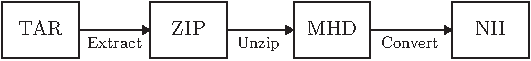
\includegraphics[width=\linewidth]{figure/conversion.pdf}
  \caption{Dataset conversion from \gls{mhd} to \gls{nifti} format.
	}\label{fig:conversion}
\end{figure}

We were able to co-register the modalities using \cite{SPM12} and the
highest interpolation order. In the same step we also resliced the volumes
to have a homogenous voxel size as the RIRE dataset has only a low resolution
in the sagittal plane.

Finally we used \cite{Nibabel} to load the aligned volumes and convert them
into Tensorflow's tfrecord format and split them into a validation set of
4 and a training set of 13 patients. Inside the tensorflow input pipeline
we normalized the value range of each volume to $[0,1]$. For two dimensional
models we padded the horizontal slices to $384\times384$. For three
dimensional models we used $260\times340\times360$ (Depth x Height x Width).

\subsection{Network}

As generative adversarial networks we decided to use pix2pix \cite{Isola16}
as it has already shown great results in the task of color image to image
translation and context-aware 3d synthesis \cite{Nie16} which uses a simpler
generator but accounts for 3d structures.

As convolutional encoder-decoder network we chose u-net \cite{Ronneberger15}
as it was able to compete with much larger models in the task of semantic
segmentation \cite{Badrinarayanan15}. Further our implementation of pix2pix
uses u-net as generator network, hence we are able to evaluate the impact
of the adversarial min-max approach.

Eventually we want to evaluate a new network and training approach novel to
medical computer vision \cite{Karras17}.

\subsubsection{U-Net}


\subsubsection{Pix2Pix}

\subsubsection{3D Synthesis}

\subsection{Losses}

\subsubsection{Distance Losses}

As norm losses we refer to the mean absolute error ($L1$ loss) and the
mean squared error ($L2$ loss).

\subsubsection{Gradient Losses}

The gradient (difference) loss is used in the framework of context-aware
3d synthesis \cite{Nie16} in addition to the norm loss.

\subsubsection{Signal Losses}

From signal processing PSNR, SSE...

\subsubsection{Adversarial Loss}

Least-squared adversarial loss, standard adversarial loss. BEGAN loss ?


\subsection{Augmentation}

\subsubsection{Random Crop}
\subsubsection{Rotation}
\subsubsection{Contast Adjustment}

